\section{DIP开发者激励协议}
\label{sec:dip}

在星云链中,我们提出面向智能合约开发者的DIP(Developer Incentive Protocol 开发者激励协议),周期性对星云链生态中所有智能合约的价值做评估,通过星云币的奖励来感谢为生态助力的优秀开发者。

DIP的设计借助周活跃用户价值总和的概念,每周进行一次,和Nebulas Rank计算周期一致。对于智能合约C,假设本周活跃账户地址集合为wad(weekly active addresses),其中根据第六章的Nebulas Rank分数,计算周活跃地址的NR之和作为合约C的贡献值。

\begin{align}
Score(C)=\sum_{addr \in wad}NR(addr)
\end{align}

每周贡献值排名Top N的智能合约开发者将按比例瓜分M个星云币作为奖励,为了避免恶意刷榜,DIP的分配曲线被设计得较为平均。

\begin{align}
Coin(C) =kln(N+1-Rank(C))+b
\end{align}

\begin{figure}[htbp] 
\centering
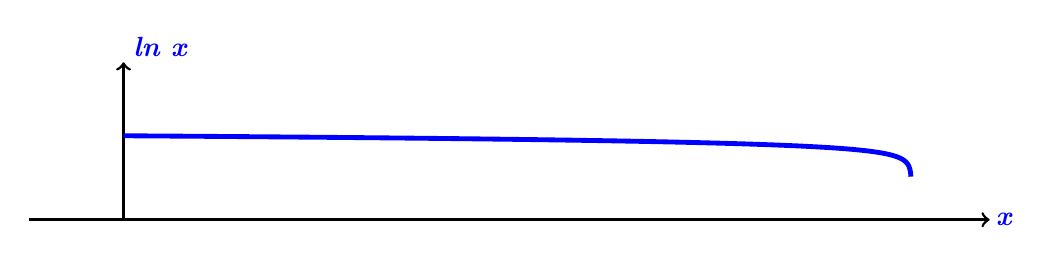
\begin{tikzpicture}
\coordinate (OR) at (0.00, 0.00);
\coordinate (LX) at (-1.20, 0.00); % left x
\coordinate (RX) at (11.00, 0.00); % right x
\coordinate (BY) at (0.00, 0.00); % bottom y
\coordinate (TY) at (0.00, 2.00); % top y
\draw[->][line width=1.00pt] (LX) -- (RX);
\node[blue] at (11.2,0) {\textbf{\textit{x}}};
\draw[->][line width=1.00pt] (BY) -- (TY);
\node[right,blue] at (0, 2.2) {\textbf{\textit{ln x}}};
  \draw[blue, line width=1.75pt, domain=0:10.00,samples=3000] plot[smooth](\x, {.066598275 * ln(3001-\x * 300) + .533210267});

\end{tikzpicture}
\label{fig:dip}
\caption{N=3000, M=3000}
\end{figure}

为了鼓励星云链生态智能合约的多样性,DIP规定每个智能合约同一个版本最多可以接受K次奖励,当使用星云原力对合约做版本更新后,新版本将可以再次接受最多K次奖励。

DIP的奖励将会由各个节点单独计算发放,假设星云链平均每S秒出一个区块,那么每隔24*7*3600/S个区块,所有节点将会计算一次DIP的奖励,并且发给对应的智能合约的提币地址中。
